\documentclass[11pt,twocolumn]{article}
\usepackage{graphicx}
\setlength{\columnsep}{1cm}
\title{Algorithmic Notes For ICPC 2021}
\author{Oscar Skean}
\date{March 2022}

\usepackage[margin=0.75in]{geometry}
\graphicspath{ {./images/} }

\begin{document}
\maketitle

\section{Template}
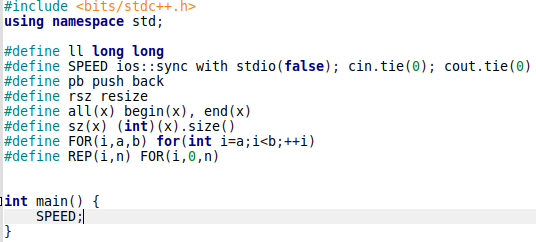
\includegraphics[scale=0.4]{template}

\section{Data Structures}
\subsection{Segment Tree}

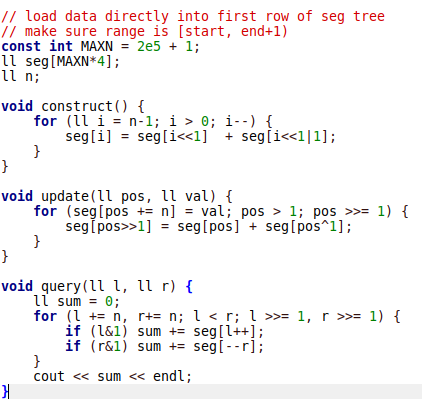
\includegraphics[scale=0.4]{segmenttree}

\subsection{Minimum Sparse}

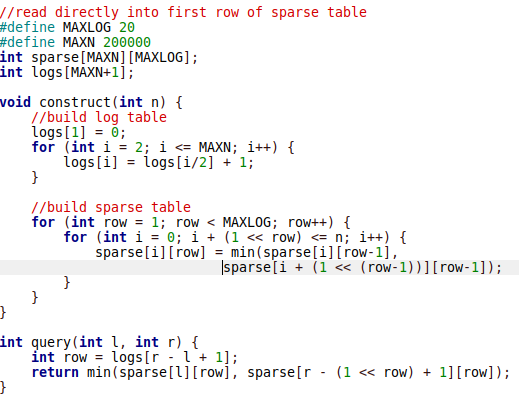
\includegraphics[scale=0.4]{sparsemin}

\subsection{Binary Jumping}

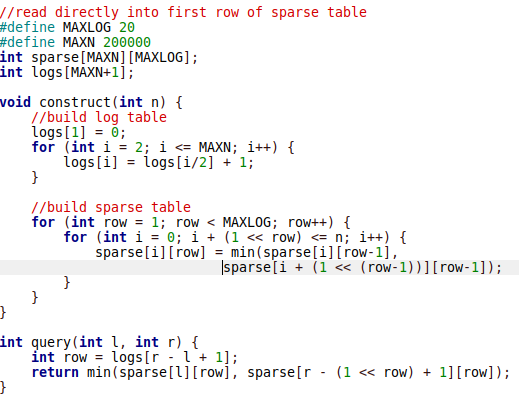
\includegraphics[scale=0.4]{sparsemin}

\section{Graph Algorithms}
\subsection{DFS with Cycle Detection}
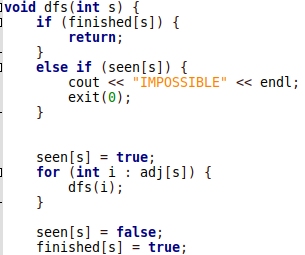
\includegraphics[scale=0.5]{dfs}
\subsection{BFS}
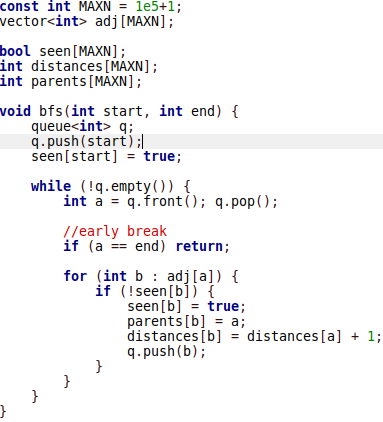
\includegraphics[scale=0.5]{bfs}
\subsection{BFS Route Reconstruction}
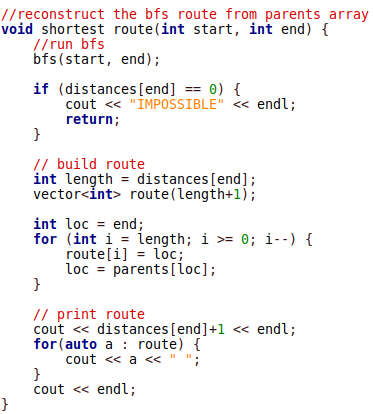
\includegraphics[scale=0.5]{bfsroutes}
\subsection{Djikstra}
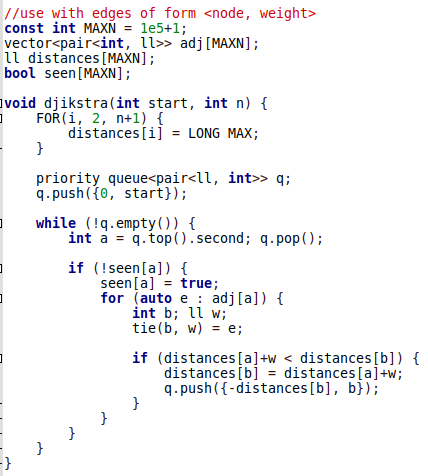
\includegraphics[scale=0.5]{djikstra}
\subsection{Bellman-Ford}

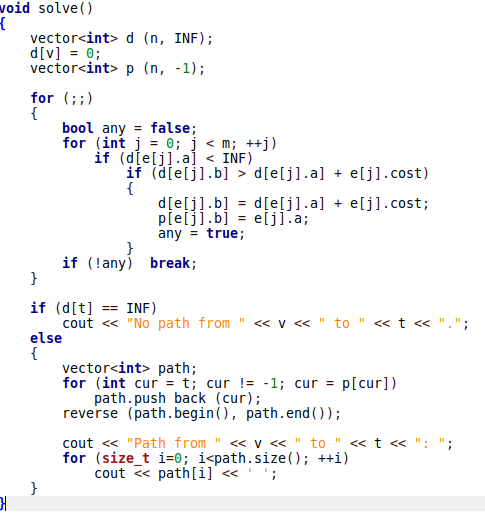
\includegraphics[scale=0.5]{bellmanford}

\subsection{Bellman-Ford with Negative Cycle Check}
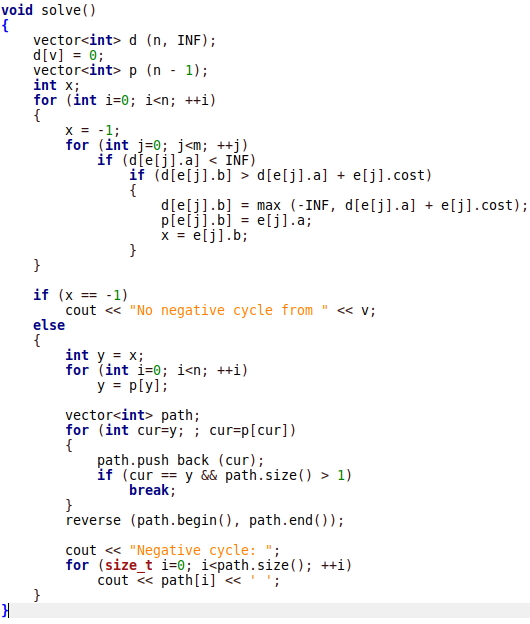
\includegraphics[scale=0.5]{bellmanfordneg}
\subsection{Floyd-Warshall}
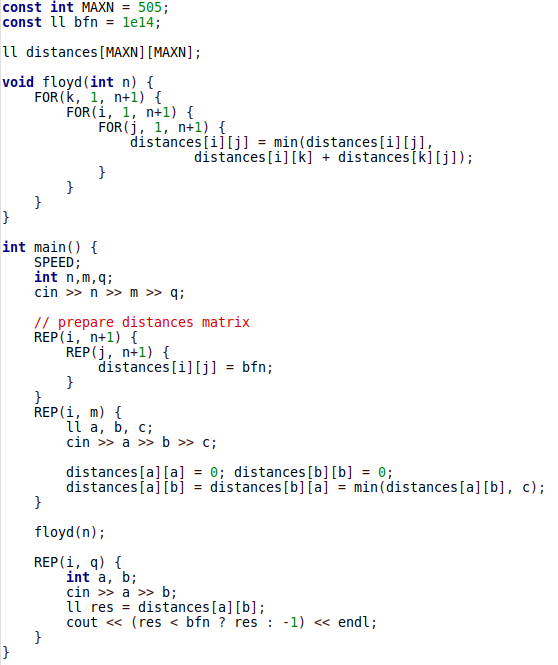
\includegraphics[scale=0.4]{floyd}
\subsection{Find Bridges of Graph}
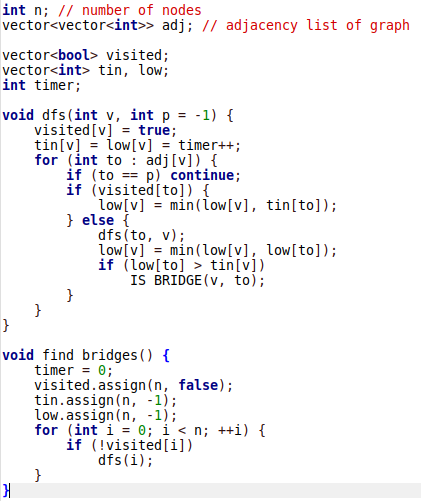
\includegraphics[scale=0.5]{bridges}
\subsection{Topological Sort}
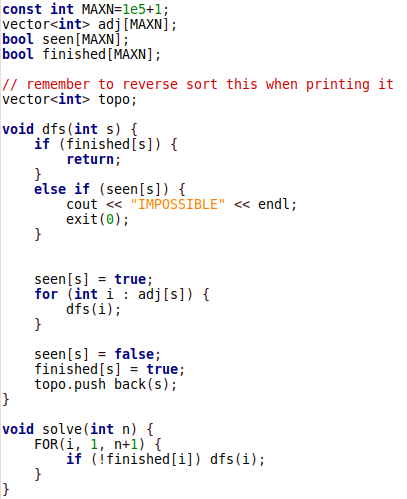
\includegraphics[scale=0.5]{topological}
\subsection{Kruskal with DSU}
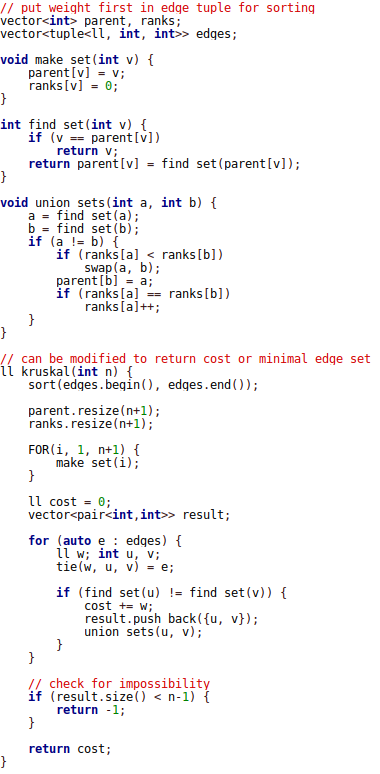
\includegraphics[scale=0.5]{kruskal}

\subsection{Connected Components}
For counting, use DFS and increment whenever the recursive call is completely finished. For listing, keep a vector that gets appended to during DFS. Print the vector, then reset it for the next component.

\subsection{Strongly Connected Components}
For counting, use DFS and increment whenever the recursive call is completely finished. For listing, keep a vector that gets appended to during DFS. Print the vector, then reset it for the next component.

\subsection{Bipartite Check}

\subsection{Maximum Flow}

\subsection{Bipartite Matching}

\subsection{Number of Paths of Fixed Length}

\subsection{2SAT}

\subsection{TSP}

\subsection{Lowest Common Ancestor}

\subsection{Eulerian Path}

\subsection{Hamiltonian Path}

\section{Dynamic Programming}
\subsection{Longest Increasing Subseqeuence}

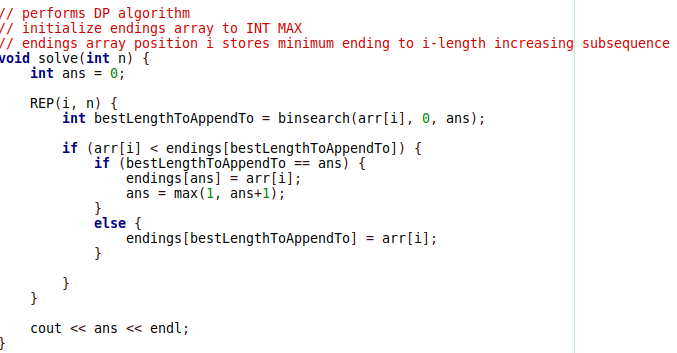
\includegraphics[scale=0.5]{lis}

\subsection{Edit Distance}
\subsection{Coins Problem}
\subsection{Knapsack}
\subsection{Rod Cutting}
\subsection{Counting Tilings}

\section{Number Theoretic}
\subsection{Primality Testing}

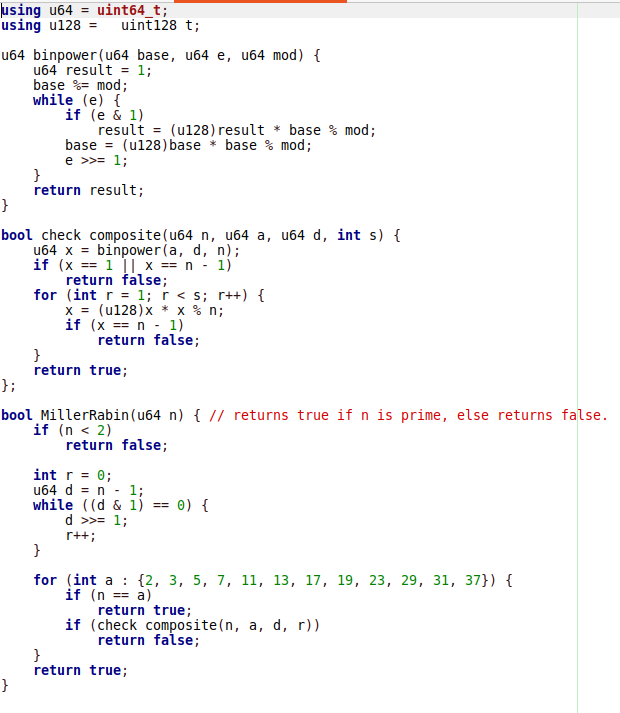
\includegraphics[scale=0.5]{millerrabin}

\subsection{Euler Totient}
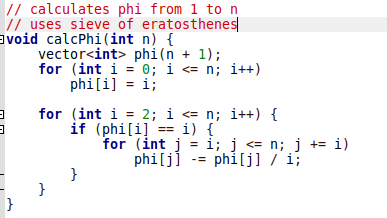
\includegraphics[scale=0.5]{eulertotient}

\subsection{Inclusion Exclusion}

\section{Strings}
\subsection{String Hashing}

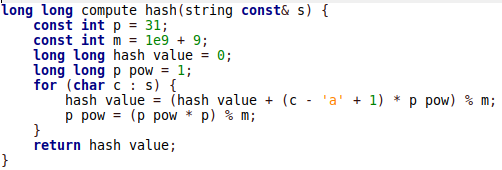
\includegraphics[scale=0.5]{hashing}

\subsection{Count unique strings in array}

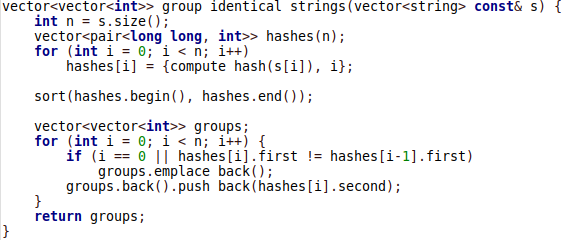
\includegraphics[scale=0.4]{identicalstrings}

\subsection{Count unique substrings of string}
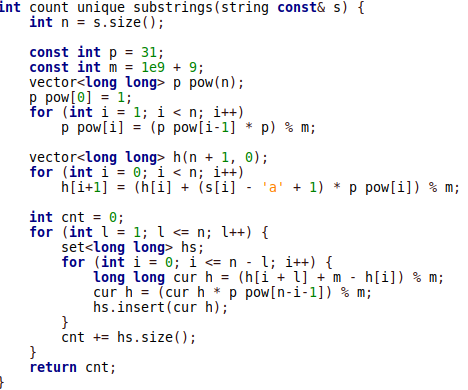
\includegraphics[scale=0.5]{uniquesubstrings}

\subsection{RabinKarp: String matching}
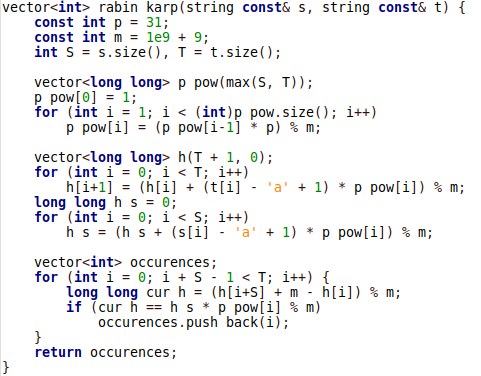
\includegraphics[scale=0.5]{rabinkarp}

\subsection{Knuth-Morris-Pratt}
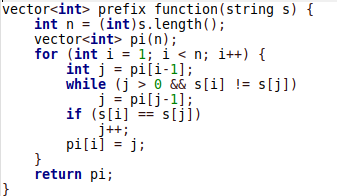
\includegraphics[scale=0.5]{kmp}

Uses:
1) Check if t is in s. Run KMP with the string s+\#+t.

\subsection{Manacher Palindroms}
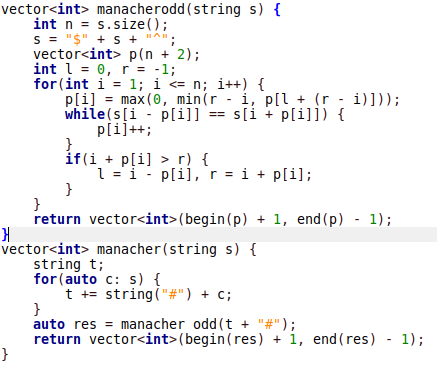
\includegraphics[scale=0.5]{manacher}


\section{Miscellaneous}
\subsection{Binary Search}

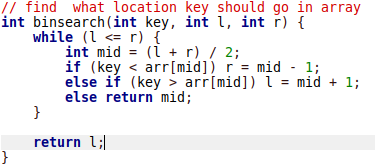
\includegraphics[scale=0.5]{binsearch}

\subsection{Binary Exponentiation}

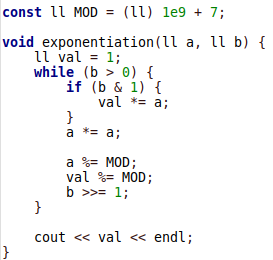
\includegraphics[scale=0.5]{binexp}

\subsection{Gray Code}

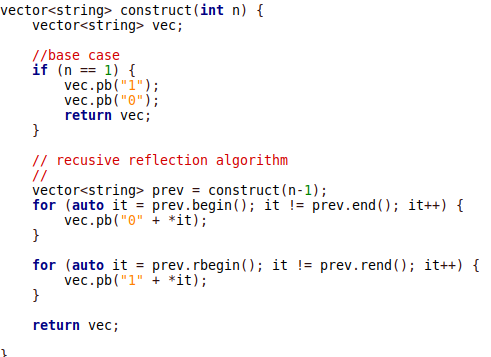
\includegraphics[scale=0.5]{graycode}

\subsection{Towers of Hanoi}
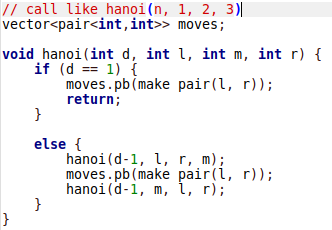
\includegraphics[scale=0.5]{hanoi}

\subsection{Expression Parsing}

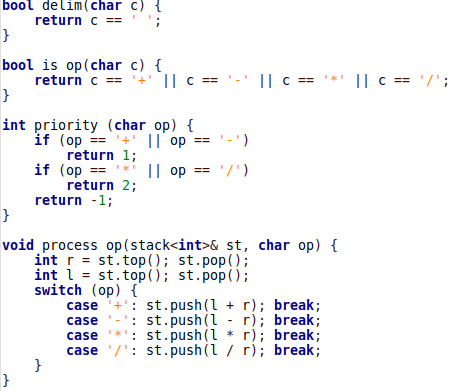
\includegraphics[scale=0.5]{parsea}

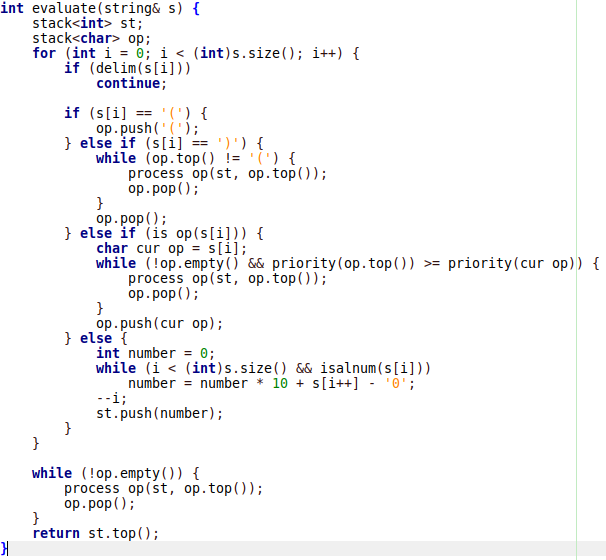
\includegraphics[scale=0.4]{parseb}

\subsection{Balanced Sequences}

\subsection{Korder Statistic}
C++ standard library has this implemented already. The function is called $nth\_element$.

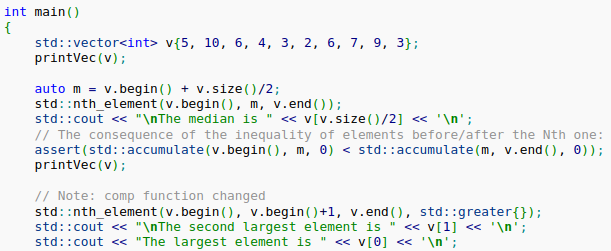
\includegraphics[scale=0.4]{nthelement}

\subsection{Josephus Queries}

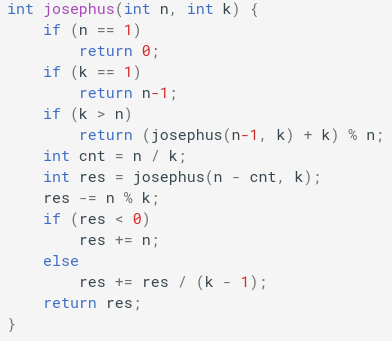
\includegraphics[scale=0.5]{quickjosephus}

\subsection{Convex Hull}
\end{document}
